\section[Разработка структуры БД]{РАЗРАБОТКА СТРУКТУРЫ БАЗЫ ДАННЫХ}
\label{sect:db_structure}

В данном разделе рассматривается процесс проектирования разрабатываемого
интернет-магазина.

В подразделе~\ref{sub:db_structure_theory} даны фундаментальные определения теории
баз данных, необходимые для понимания излагаемого материала.

Далее, в подразделах~\ref{sub:db_structure_aims}~и~\ref{sub:db_structure_stages}
приведены цели, задачи, основные этапы проектирования баз данных.
В подразделах~\ref{sub:db_structure_concept_design},
\ref{sub:db_structure_logical_design}~и~\ref{sub:db_structure_physical_design}
подробно раскрыт каждый из этапов проектирования баз данных.

В процессе проектирования базы данных использовалось средство автоматизированного
проектирования CA ERWin.
Для построения диаграммы прецедентов было использовано CASE-средство
Enterprise Architect, разработанное компанией Sparx Systems.

\subsection{Основные определения}
\label{sub:db_structure_theory}

\textit{База данных} --- совместно используемый набор логически связанных данных
(и описание этих данных), предназначенный для удовлетворения информационных
потребностей организации.

\textit{Система управления базами данных (СУБД)} --- программное обеспечение,
с помощью которого пользователи могут определять, создавать и поддерживать базу данных,
а также осуществлять к ней контролируемый доступ~\cite{konnolli03}.

\textit{Модель данных} --- это абстрактное, самодостаточное,
логическое определение объектов, операторов и прочих элементов,
в совокупности составляющих абстрактную  машину доступа к данным,
с которой взаимодействует пользователь.

\textit{Реляционная модель данных} состоит из трех частей:
\begin{itemize}
\item
  \textit{структурная часть} описывает, какие объекты рассматриваются
  реляционной моделью. Единственной структурой данных, используемой
  в реляционной модели, являются \textit{нормализованные отношения}.
\item
  \textit{целостная часть} описывает ограничения специального вида,
  которые должны выполняться для любых отношений в любых реляционных базах данных.
  Это целостность сущностей и целостность внешних ключей.
\item
  \textit{манипуляционная часть} описывает два эквивалентных способа
  манипулирования реляционными данными --- \textit{реляционную алгебру} и
  \textit{реляционное исчисление}.
\end{itemize}

Процесс преобразования отношений базы данных к виду, отвечающему нормальным формам,
называется \textit{нормализацией}.

Переменная отношения находится в \textit{первой нормальной форме} тогда и только
тогда, когда в любом допустимом значении этой переменной отношения каждый её кортеж
содержит только одно значение для каждого из атрибутов.

Переменная отношения находится во \textit{второй нормальной форме} тогда и только тогда,
когда она находится в первой нормальной форме и каждый неключевой атрибут
неприводимо зависит от ее первичного ключа.

Переменная отношения находится в \textit{третьей нормальной форме} тогда и только
тогда, когда она находится во второй нормальной форме и в ней отсутствуют транзитивные
зависимости~\cite{date05}.

Переменная отношения находится в \textit{нормальной форме Бойса-Кодда} тогда и только тогда,
когда каждый её детерминант является потенциальным ключом~\cite{konnolli03}.

Необходимо отметить, что существуют нормальные формы более высоких порядков, но
на практике они используются реже.

\subsection{Цели и задачи проектирования базы данных}
\label{sub:db_structure_aims}

Основные \textit{цели проектирования баз данных:}
\begin{itemize}
  \item централизация данных;
  \item сокращение избыточности и дублирования данных;
  \item обеспечение целостности БД;
  \item обеспечение возможности получения данных по всем необходимым запросам.
\end{itemize}

\textit{Задача проектирования базы данных} в общем случае формулируется следующим образом: выбрать
подходящую структуру для заданного массива данных, которое требуется поместить в базу данных.
Иначе говоря, нужно решить вопрос, какие необходимы базовые переменные отношения и какой
набор атрибутов они должны включать~\cite{date05}.

\subsection{Этапы проектирования баз данных}
\label{sub:db_structure_stages}
Как правило на практике выделяют три этапа проектирования баз данных:
\begin{itemize}
  \item концептуальное проектирование;
  \item логическое проектирование;
  \item физическое проектирование.
\end{itemize}

Рассмотрим каждый из этапов подробнее.

\textit{Концептуальное (инфологическое) проектирование} --- создание концептуального
представления базы данных, включающее определение типов важнейших сущностей и существующих
между ними связей и атрибутов.

Концептуальное проектирование базы данных начинается с создания концептуальной
модели данных предприятия, полностью независимой от любых деталей
реализации. К последним относятся выбранный тип СУБД,
состав программ приложения, используемый язык программирования, конкретная аппаратная
платформа, вопросы производительности и любые другие физические особенности реализации.

\textit{Логическое (даталогическое) проектирование} --- преобразование
концептульного представления в логическую структуру базы данных,
включая проектирование отношений.

Логическое проектирование базы данных заключается в преобразовании
концептуальной модели данных в логическую модель данных предприятия с учетом
выбранного типа СУБД (например, предполагается использование
реляционной СУБД). Логическая модель данных является источником информации
для этапа физического проектирования. Она предоставляет разработчику
физической модели данных средства проведения всестороннего анализа различных
аспектов работы с данными, что имеет исключительно важное значение для
выбора действительно эффективного проектного решения.

\textit{Физическое проектирование} --- принятие решения о том, как логическая модель
будет физически реализована (с помощью таблиц) в базе данных, создаваемой
с использованием выбранной СУБД.

Физическое проектирование базы данных предусматривает принятие разработчиком
окончательного решения о способах реализации создаваемой базы. Поэтому
физическое проектирование обязательно производится с учетом всех особенностей
используемой СУБД. Между этапами физического и логического проектирования
всегда имеется определенная обратная связь, поскольку решения,
принятые на этапе физического проектирования с целью повышения производительности
разрабатываемой системы, могут потребовать определенной корректировки логической
модели данных~\cite{konnolli03}.

\subsection{Концептуальное проектирование}
\label{sub:db_structure_concept_design}

\paragraph{}
Разрабатываемый интернет-магазин должен предоставлять актуальную информацию о
имеющихся в продаже товарах конечному пользователю, позволять совершать покупки.

На рисунке~\ref{fig:use_case} изображена диаграмма прецедентов
разрабатываемого интернет-магазина.

\begin{figure}[h]
  \centering
  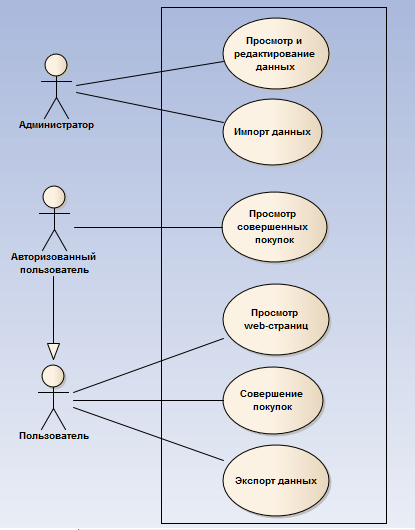
\includegraphics[width=100mm]{pic/use_case.png}
  \caption{Диаграмма прецедентов \\ проектируемого интернет-магазина}
  \label{fig:use_case}
\end{figure}

Так, \textit{пользователь} имеет возможность просматривать все веб-страницы,
совершать покупки, а также экспортировать данные о товарах в файлы формата xml.

Совершив покупку пользователь автоматически регистрируется в системе,
тем самым переходя в группу \textit{авторизованных пользователей}.
Зарегистрированные в системе пользователи могут просматривать сделанные ранее покупки,
получать назначаемые администратором скидки.

\textit{Администратор} разрабатываемого интернет-магазина просматривает
и редактирует каталог товаров. Также он имеет возможность
пополнения каталога товаров путём загрузки информации в базу данных с
локального носителя.

\paragraph{}
Пополнение каталога товаров разрабатываемого интернет-магазина должно осуществляться
только администратором путём использования веб-интерфейса разрабатываемого
интернет-магазина, или путём загрузки информации
о товарах напрямую в базу данных используя файлы с расширением xml.

\paragraph{}
Исходя из описанных выше минимальных требований к разрабатываемой
системе, можно выделить следующие необходимые объекты-сущности:
\begin{itemize}
  \item <<велосипеды>> --- хранит полное описание велосипедов;
  \item <<велосипеды в наличии>> --- хранит информацию о велосипедах, находящихся в наличии;
  \item <<заказы велосипедов>> --- хранит информацию о заказах, ожидающих выполнения;
  \item <<архив заказов>> --- сохраняет информацию о совершенных пользователями
    покупках;
  \item <<пользователи>> --- хранит информацию о всех зарегистрированных пользователях.
\end{itemize}

Отметим, что необходимость существования сущности <<архив заказов>> в разрабатываемой
системе обусловлена стремлением повысить скорость работы системы. Так, при просмотре
архивных данных объект <<заказы велосипедов>> нагружаться не будет.

\pagebreak

На рисунке~\ref{fig:ER_model} представлена ER-модель
разрабатываемого интернет-магазина.

\begin{figure}[h]
  \centering
  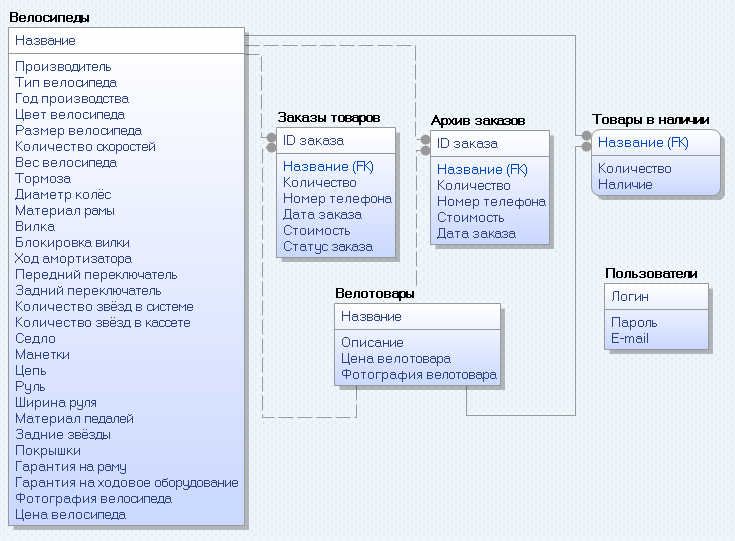
\includegraphics[width=150mm]{pic/ER.png}
  \caption{ER-модель проектируемого интернет-магазина}
  \label{fig:ER_model}
\end{figure}

Опишем отношения между сущностями разрабатываемой базы данных на основе спроектированной ER-модели.

Каждому объекту <<Велосипеды в наличии>> соответствует конкретный экземпляр
сущности <<Велосипеды>> (тип отношения --- \textit{<<один-к-одному>>});

%Объект <<Велосипеды в наличии>> может быть связан с одним конкретным объектом
%типа <<Велосипеды>> или <<Велотовары>> (отношения типа \textit{один-к-одному});

Нескольким объектам сущности <<Заказы велосипедов>> и <<Архив заказов>> может
соответствовать конкретный объект сущности <<Велосипеды>> (тип отношения ---
\textit{<<многие-к-одному>>}).

Один пользователь может сделать несколько покупок велосипедов. Таким образом
объекты сущности <<Заказы велосипедов>>, <<Архив заказов>> и <<Пользователи>>
состоят в отношении \textit{<<многие-к-одному>>}.

%Объекты <<Заказы велосипедов>> и <<Архив заказов>> могут быть связаны
%с конкретными объектами типа <<Велосипеды>> или <<Велотовары>>. Каждому
%объекту <<Заказы товаров>> и <<Архив заказов>> соответствует конкретный объект
%типа <<Пользователи>> (отношения типа \textit{один-к-одному}).

\pagebreak

\subsection{Логическое проектирование}
\label{sub:db_structure_logical_design}

\paragraph{}
На основе ER-модели, спроектированной в подразделе~\ref{sub:db_structure_concept_design},
построим логическую модель базы данных. Схема логической модели
представлена на рисунке~\ref{fig:logical_model}.
\begin{figure}[h]
  \centering
  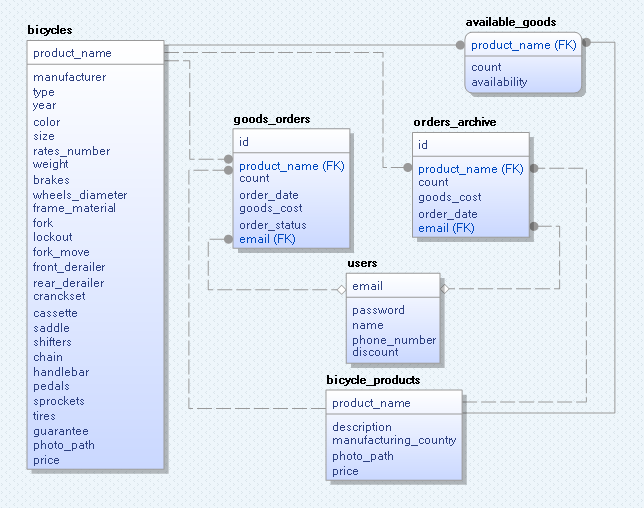
\includegraphics[width=150mm]{pic/logical_model.png}
  \caption{Логическая модель проектируемой базы данных}
  \label{fig:logical_model}
\end{figure}

Далее рассмотрим каждую из представленных на рисунке~\ref{fig:logical_model} сущностей
подробнее. Приведём соответствия названий атрибутов отношений ER и логической модели.
Для каждого из атрибутов укажем тип хранимых данных.

\pagebreak

\paragraph{}
Объекту <<Велосипеды>> соответствует отношение \textit{<<bicycles>>}, схема которого приведена в
таблице~\ref{tbl:bicycles_scheme}.
\begin{table}[h!]
  \caption{Схема отношения \textit{<<bicycles>>}}
  \label{tbl:bicycles_scheme}
  \small{
    \centering
    \begin{tabular}{| p{0.32\textwidth} | p{0.29\textwidth} | p{0.3\textwidth} |}
      \hline
      Название атрибута в \newline логической модели &
      Название атрибута в \newline отношении &
      Тип хранимых данных \\

      \hline
      ID & id & BIGINT \\

      \hline
      Название & product\_name & VARCHAR(255) \\

      \hline
      Производитель & manufacturer & VARCHAR(255) \\

      \hline
      Тип велосипеда & type & VARCHAR(20) \\

      \hline
      Год производства & year & YEAR \\

      \hline
      Цвет велосипеда & color & VARCHAR(20) \\

      \hline
      Размер велосипеда & size & CHAR \\

      \hline
      Количество скоростей & rates\_number & TINYINT(4) \\

      \hline
      Вес велосипеда & weight & DOUBLE \\

      \hline
      Тормоза & brakes & VARCHAR(255) \\

      \hline
      Диаметр колёс & wheels\_diameter & UNSIGNED TINYINT \\

      \hline
      Материал рамы & frame\_material & VARCHAR(50) \\

      \hline
      Вилка & fork & VARCHAR(255) \\

      \hline
      Блокировка вилки & lockout & TINYINT(1) \\

      \hline
      Ход амортизатора & fork\_move & UNSIGNED TINYINT \\

      \hline
      Передний переключатель & front\_derailer & VARCHAR(255) \\

      \hline
      Задний переключатель & rear\_derailer & VARCHAR(255) \\

      \hline
      Система & cranckset & VARCHAR(255) \\

      \hline
      Кассета & cassette & VARCHAR(255) \\

      \hline
      Седло & saddle & VARCHAR(255) \\

      \hline
      Манетки & shifters & VARCHAR(255) \\

      \hline
      Цепь & chain & VARCHAR(255) \\

      \hline
      Руль & handlebar & VARCHAR(255) \\

      \hline
      Педали & pedals & VARCHAR(255) \\

      \hline
      Покрышки & tires & VARCHAR(255) \\

      \hline
      Гарантия & guarantee & VARCHAR(255) \\

      \hline
      Фотография велосипеда & photo\_path & VARCHAR(255) \\

      \hline
      Цена & price & DOUBLE \\

      \hline
    \end{tabular}
  }
\end{table}

Рассмотрим некоторые атрибуты отношения \textit{<<bicycles>>} подробнее:
\begin{itemize}
  \item \textit{<<id>>} является первичным ключом;
  \item \textit{<<size>>} может принимать значения <<XS>>, <<S>>, <<M>>, <<L>>, <<XL>> или <<XXL>>;
  \item \textit{<<weight>>} указывается в килограммах и обозначает вес велосипеда
    без педалей в соответствии с международными стандартами;
  \item \textit{<<wheels\_diameter>>} хранит значение, указываемое в дюймах;
  \item \textit{<<fork\_move>>} хранит значение, указываемое в миллиметрах.
\end{itemize}

%\paragraph{}
%Объекту <<Велотовары>> соответствует отношение \textit{<<bicycle\_products>>}, схема которого приведена в
%таблице~\ref{tbl:bicycle_products_scheme}.
%\begin{table}[h!]
%  \caption{Схема отношения \textit{<<bicycle\_products>>}}
%  \label{tbl:bicycle_products_scheme}
%  \small{
%    \centering
%    \begin{tabular}{| p{0.32\textwidth} | p{0.29\textwidth} | p{0.3\textwidth} |}
%      \hline
%      Название атрибута в \newline логической модели &
%      Название атрибута в \newline отношении &
%      Тип хранимых данных \\
%
%      \hline
%      Название & product\_name & VARCHAR(255) \\
%
%      \hline
%      Описание & description & VARCHAR(255) \\
%
%      \hline
%      Фотография & photo\_path & VARCHAR(255) \\
%
%      \hline
%      Страна производитель & manufacturing\_country & VARCHAR(255) \\
%
%      \hline
%      Цена & price & FLOAT \\
%
%      \hline
%    \end{tabular}
%  }
%\end{table}

%Атрибут \textit{<<product\_name>>} является первичным ключом отношения \textit{<<bicycle\_products>>},
%атрибут \textit{<<photo\_path>>} хранит информацию о расположении фотографии велотовара
%на жестком диске.

\paragraph{}
Объекту <<Велосипеды в наличии>> соответствует отношение \textit{<<available\_bicycles>>},
схема которого приведена в таблице~\ref{tbl:available_bicycles_scheme}.
\begin{table}[h!]
  \caption{Схема отношения \textit{<<available\_bicycles>>}}
  \label{tbl:available_bicycles_scheme}
  \small{
    \centering
    \begin{tabular}{| p{0.32\textwidth} | p{0.29\textwidth} | p{0.3\textwidth} |}
      \hline
      Название атрибута в \newline логической модели &
      Название атрибута в \newline отношении &
      Тип хранимых данных \\

      \hline
      ID & id & BIGINT(20) \\

      \hline
      ID велосипеда & bicycle\_id & BIGINT(20) \\

      \hline
      Количество & count & INT \\

      \hline
      Наличие & availability & TINYINT(1) \\

      \hline
    \end{tabular}
  }
\end{table}

Атрибут \textit{<<id>>} является первичным ключом, \textit{<<bicycle\_id>>} --- внешним ключом
отношения \textit{<<available\_bicycles>>}, ссылаясь на таблицы \textit{<<bicycles>>}.

\paragraph{}
Объекту <<Заказы велосипедов>> соответствует отношение \textit{<<orders>>},
схема которого приведена в таблице~\ref{tbl:orders_scheme}.
\begin{table}[h!]
  \caption{Схема отношения \textit{<<orders>>}}
  \label{tbl:orders_scheme}
  \small{
    \centering
    \begin{tabular}{| p{0.32\textwidth} | p{0.29\textwidth} | p{0.3\textwidth} |}
      \hline
      Название атрибута в \newline логической модели &
      Название атрибута в \newline отношении &
      Тип хранимых данных \\

      \hline
      ID & id & BIGINT \\

      \hline
      ID велосипеда & bicycle\_id & BIGINT \\

      \hline
      Количество & count & INT \\

      \hline
      Дата заказа & order\_date & DATE \\

      \hline
      Стоимость товаров & goods\_cost & DOUBLE \\

      \hline
      Статус заказа & order\_status & VARCHAR(255) \\

      \hline
      ID пользователя & user\_id & BIGINT(20) \\

      \hline
    \end{tabular}
  }
\end{table}

Атрибут \textit{<<id>>} хранит уникальные целые значения и является первичным ключом.
Атрибут \textit{<<bicycle\_id>>} является внешним ключом
и ссылается на таблицу \textit{<<bicycles>>}.
Атрибут \textit{<<user\_id>>} также является внешним ключом и ссылается
на таблицу \textit{<<users>>}.

\paragraph{}
Объекту <<Архив заказов>> соответствует отношение \textit{<<orders\_archive>>}, схема которого приведена в
таблице~\ref{tbl:orders_archive_scheme}.
\begin{table}[h!]
  \caption{Схема отношения \textit{<<orders\_archive>>}}
  \label{tbl:orders_archive_scheme}
  \small{
    \centering
    \begin{tabular}{| p{0.32\textwidth} | p{0.29\textwidth} | p{0.3\textwidth} |}
      \hline
      Название атрибута в \newline логической модели &
      Название атрибута в \newline отношении &
      Тип хранимых данных \\

      \hline
      ID & id & BIGINT(20) \\

      \hline
      ID велосипеда & bicycle\_id & BIGINT(20) \\

      \hline
      Количество & count & INT \\

      \hline
      Дата заказа & order\_date & DATE \\

      \hline
      Стоимость товаров & goods\_cost & DOUBLE \\

      \hline
      ID пользователя & user\_id & BIGINT(20) \\

      \hline
    \end{tabular}
    }
\end{table}

Атрибуты отношения \textit{<<orders\_archive>>} идентичны атрибутам
\textit{<<orders>>}, представленным в таблице~\ref{tbl:orders_scheme}.

\paragraph{}

Объекту <<Пользователи>> соответствует отношение \textit{<<users>>}, схема которого приведена в
таблице~\ref{tbl:users_scheme}.

\begin{table}[h]
  \caption{Схема отношения \textit{<<users>>}}
  \label{tbl:users_scheme}
  \small{
    \centering
    \begin{tabular}{| p{0.32\textwidth} | p{0.29\textwidth} | p{0.3\textwidth} |}
      \hline
      Название атрибута в \newline логической модели &
      Название атрибута в \newline отношении &
      Тип хранимых данных \\

      \hline
      ID & id & BIGINT(20) \\

      \hline
      E-mail & email & VARCHAR(255) \\

      \hline
      Пароль & password & VARCHAR(255) \\

      \hline
      Имя & name & VARCHAR(20) \\

      \hline
      Номер телефона & phone\_number & VARCHAR(20) \\

      \hline
    \end{tabular}
    }
\end{table}

Атрибут \textit{<<id>>} отношения \textit{<<users>>} является первичным ключом.
Пароль пользователей хранится в зашифрованном виде.

\subsection{Физическое проектирование}
\label{sub:db_structure_physical_design}

Главной целью физического проектирования является перенос разработанной логической модели
на конкретное аппаратное и программное обеспечение. С учетом выбранной СУБД (смотри
подраздел~\ref{sub:choice_DBMS}) был выполнен данный этап проектирования.

\pagebreak
